\chapter{Network Design}
\label{chap:design}

\section{Assumptions}

Several assumptions are made in designing the network.
\begin{enumerate}
    \item There is only one source device and one destination device in the network. All other nodes are intermediate nodes.
    \item The address of the destination device is fixed.
    \item All links between neighbouring nodes are bi-directional. If a node is able to send a packet directly to a neighbour, it should be able to receive a packet directly from the neighbour.
\end{enumerate}

\section{Network Components}

\subsection{Sensinode Devices}

In this coursework, the physical node we are using is called ‘Sensinode’, which is invented and created by Sensinode Ltd, a company that focuses research on the Internet of Things(IoT). 
Sensinode’s solution enables development and support of device networks built around the IPv6 protocol and Embedded Web Services. 
The Sensinode NanoService provides end-to-end web services optimized for the constraints of M2M deployments. 

Sensinode is running on Contiki Operating System \footnote{http://www.contiki-os.org}, which provides a variety of handy and primitive APIs for building Wireless Sensor Network.
Applications running on Contiki OS are written in C programming language.

\subsection{Person Computers}
Sensinode devices in the network are connected to person computers for downloading the program and displaying the output. Although those computers are not part of the network, they play an important rule in understanding the flow of information inside the network.


\section{Roles Inside Network}
\label{sec:architecture}
There are three different roles inside the network--the Source Device, Intermediate Devices as well as the Destination Device.

\subsection{Source Device}
Source device in the routing discovery stage is as a first originator for broadcasting request message (RREQ) to other nodes, connecting other intermediate nodes to find destination node in Ad-Hoc wireless sensor network. After receiving a Reply message (RREP) from the destination node, it reads all the routing information such as route index and choose the best route to send packets. At the packet delivery stage, it is able to collect all information such as light, temperature, voltage and sent them in a single packet to the destination node through intermediate nodes. Type of data to transfer is also able to change by clicking the desired button on the source node.

\subsection{Intermediate Devices}
There are four intermediate nodes in our desired Ad-Hoc wireless sensor network. At route discovery stage, their job is receiving a broadcast from the originator and broadcast those request message (RREQ) again to other intermediate nodes until it reached destination nodes. In contrast, it will create a reverse path to carrying reply message (RREP) from destination node to source node.

\subsection{Destination Device}
The destination device is the opposite side of the originator, it works with other nodes to establish a route which works most efficient. At routing discovery stage its job is to receive the RREQ and check if itself is the destination node; if destination node confirmed it would send the RREP back to where the RREQ comes from. At the packet delivery stage, its job is receiving the packet of different readings such as temperature, light, voltage and eventually display all information that source node gathered on the screen of computers.

\section{Stage One: Route Discovery}
\label{sec:design-aodv}
Our design of route discovery is a simplified version of AODV protocol. There are two sub-stages inside route discovery--Route Request and Route Reply.

\subsection{Route Request}

When the source device needs to send a data packet to the destination and no route towards the destination is found inside its route table, the source device initiates the AODV protocol.
The source broadcasts a route discovery request (RREQ) to its neighbours, which contains a One Byte Unique Header Field, RREQ ID, and destination address.
The RREQ ID inside the packet increments by one each time a new RREQ is sent.

\begin{figure}
\centering
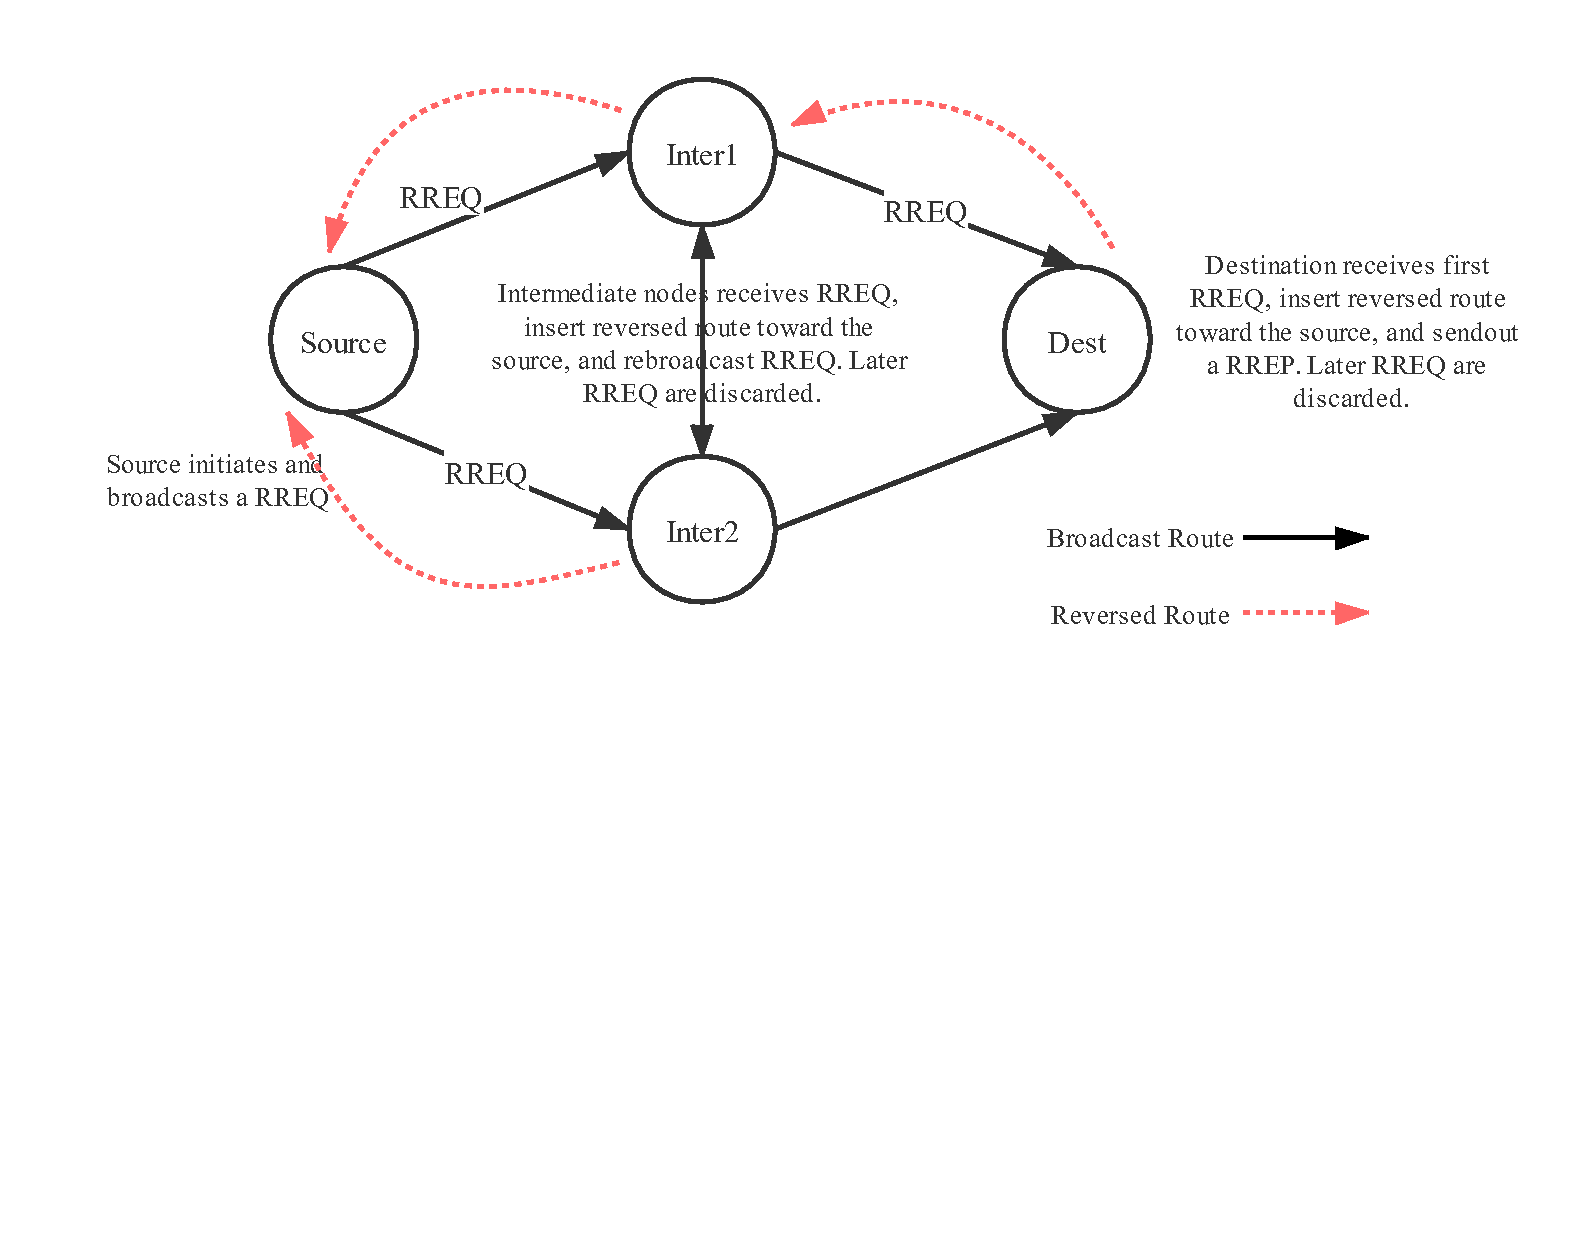
\includegraphics[width=\textwidth]{request}
\caption{Broadcasting a Request (RREQ) in AODV Protocol.}
\label{fig:request}
\end{figure}

Each intermediate node, on receiving the first RREQ, verifies the Unique Header Field, whose value should be constant 0x33, to distinguish our group's packets from others'.
If the RREQ is verfied, the intermediate node inserts a reversed route into its route table. The destination of of the route is the source device and the next hop is the node it receives the RREQ from.
The node then re-broadcasts the RREQ to its neighbours.
The node saves the address of the source and the RREQ ID as the last source and RREQ ID it receives.
The node, on receiving later RREQs of the same source and RREQ ID, discards all late-coming RREQs.


The destination device, on receiving the RREQ, likewise, verifies the Unique Header Field and inserts a reversed route into its route table.
However, it doesn't re-broadcast the RREQ.
It sends a route discovery reply (RREP) towards the source device.
The destination device saves the address of the source and the RREQ ID as the last source and RREQ ID it receives.
The destination device, on receiving later RREQs of the same source and RREQ ID, discards all late-coming RREQs.



\subsection{Route Reply}
The RREP contains a Unique Header Field, the source (destination device) addres, the destination (the source device) address and the RSSI value of the RREQ packet the destination device receives (first\_rssi).
The destination device sends out RREP to the node it receives the RREQ packet from, essentially using the route learns from the RREP packet.

\begin{figure}
\centering
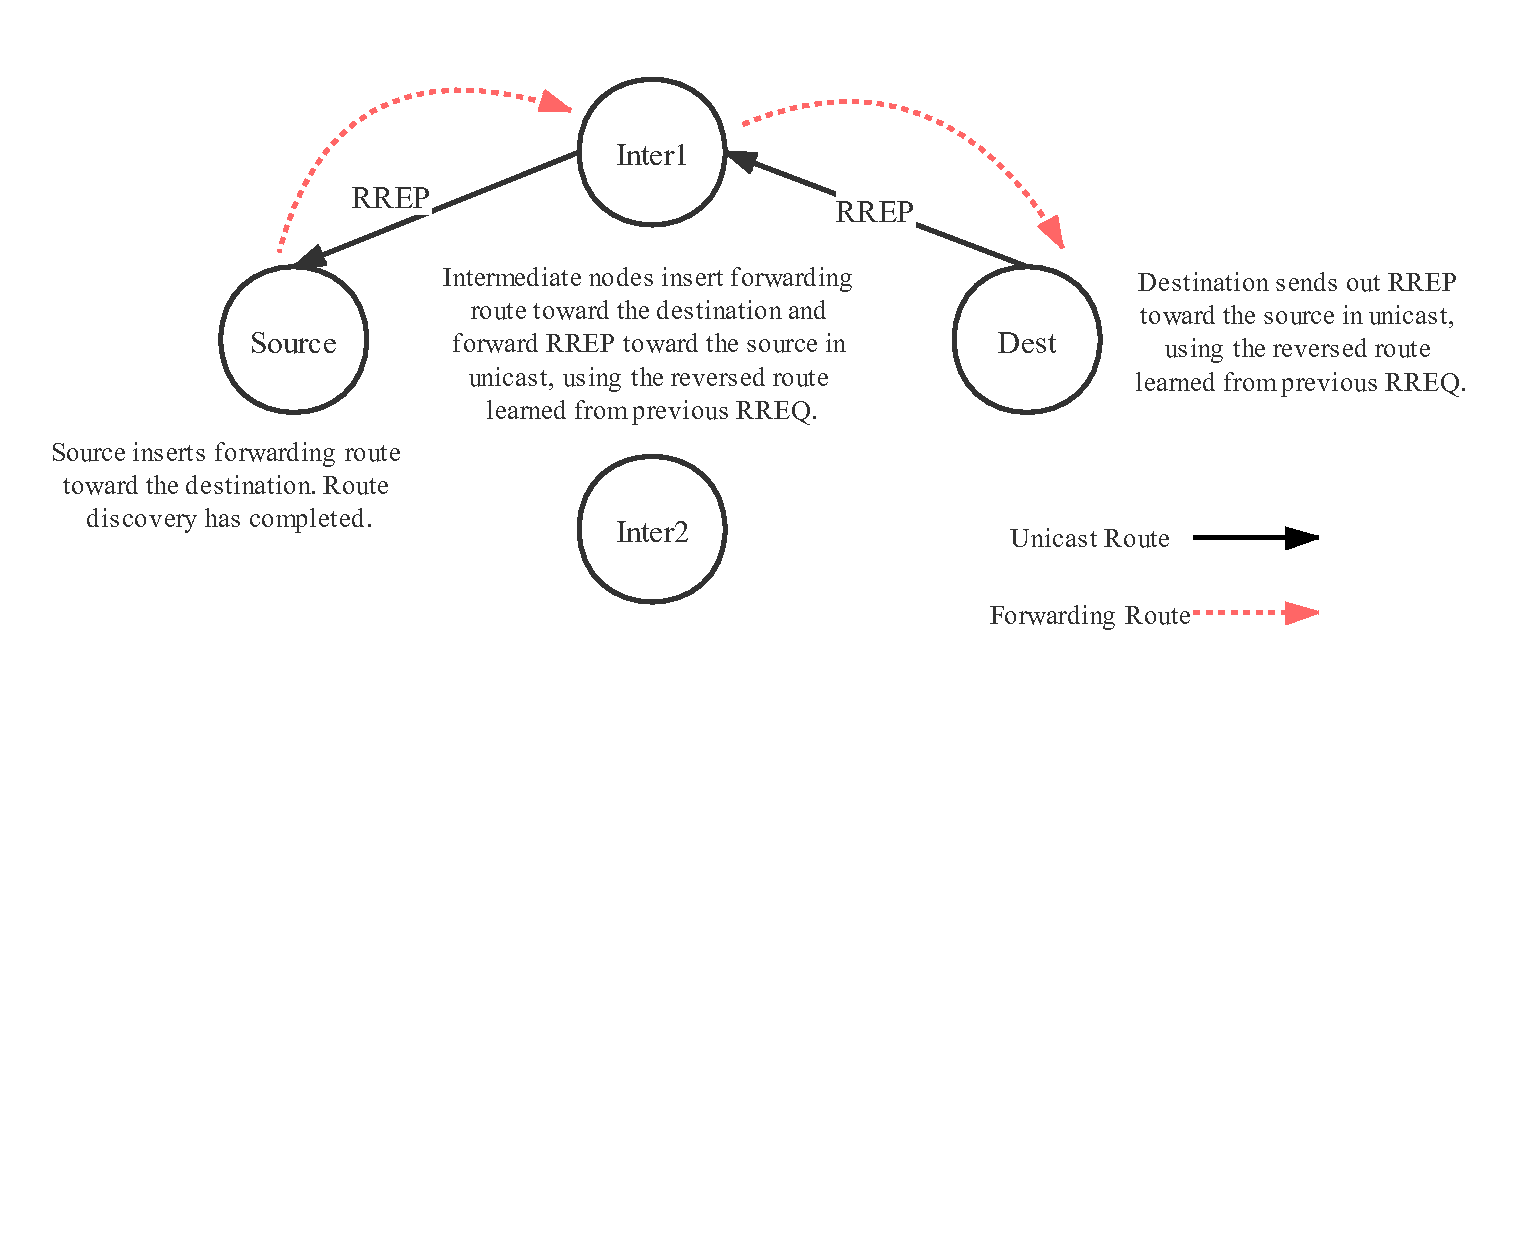
\includegraphics[width=\textwidth]{reply}
\caption{Forwarding a Reply (RREP) in AODV Protocol.}
\label{fig:request}
\end{figure}

Each node, on receiving the RREP, verifies the Unique Header Field, whose value should be a constant 0x33, to distinguish our group's packets from others'.
The node appends its address, battery level and RSSI value of the RREP packet it receives to the packet.
The node inserts a forwarding route towards the destination device into its own route table.
The destination of the route is the destination device and the next hop is the node it receives RREP from.
The route index is computed using the first\_rssi value and the appended information by previous nodes.
The node then forwards the RREP packet through the route is learns from the request stage.

The source node, on receiving the RREP, likewise, verifies the Unique Header Field, inserts a forwarding route into the route table and computes the route index.
However, it does not forwards RREP packet.
At this moment, the source node has learnt a new route towards the destination.

\subsection{Route Expiry and Renewal}
Each route learnt from AODV protocol, by default, has a lifetime of $10$ seconds.
However, if the route has been proven to be valid, the route will be renewed immediately by the node.
Concretely, if node A receives a packet from node B originated from node C, the route whose destination is node C and next hop is node B in node A's route table will be renewed right away.

If the route has been proven to be invalid, the route will be purged immediately by the node.
Concretely, if node A sends a data packet to node C through node B but doesn't receive an acknowledgement from node C, the route whose destination is node C and next hop is node B in node A's route table will be purged right away.

Route Expiry and Renewal ensures that each route is always up to date and forces the node to initiate a route discovery when a route is no longer valid.

\section{Stage Two: Data Delivery}

At this stage, for source node, it has its primary process, where every time it initiated, it will wait two seconds and then decide what type of value it is going to collect; Whether temperature/light value or battery voltage. Then it will send a packet to intermediate nodes ask them to forward to the destination node. Since it is multithreading, at packet received call-back, it will check if it is destination while a packet received. If the answer is negative, it will be looking up route table to see if destination in route table or not, it will unicast to next route entry if it finds destination in route table, or it will redo route discovery process if there is no destination in its route table. At the same time button even, handler is waiting to check which button has been clicked; If the button one has clicked the information output mode will be modified, whereas sensor value content will be modified while button two has been clicked.

As for the destination node, the job is receiving packets and displaying them on-screen of the PC. It has multi-thread as well. It will initialize event handler first, while it received a packet, it will check whether if itself is a destination. If the answer is positive, it will resolve what content that packet have, whether it is temperature/light value or battery value, and print everything on screen; if the answer is negative, it will be looking up in route table and check if it needs to unicast route entry or redo the route discovery. Simultaneously debug information handler will check if the button has pressed with button the event handler, if the button has been pressed, it will change debug output. 






